\documentclass[alsotrans]{beamerswitch}
\usepackage{iprog}

\title{Уводна лекция}

\date{4 октомври 2021 г.}

\begin{document}

\begin{frame}
  \titlepage
\end{frame}

\begin{frame}
  \frametitle{Какво е компютър?}

  Архитектура на von Neumann\\

  \begin{center}
    % TODO: диаграмата да се направи с TikZ
    \renewcommand{\arraystretch}{1.2}
    \begin{tabular}{c*4{@{}c}}
      \hhline{~~-~~}
      \multicolumn 2{@{}m{16ex}}{\multirow 2*[2ex]{\onslide<2->{%
      \basedOnImageWithAttr[1em]{12ex}{images/cpu.jpg}{CPU}{Dāvis Mosāns}{https://flic.kr/p/eKGQPJ}{\CCBY{2.0}}}}}&
      \multicolumn 1{|c|}{\cellcolor{diagramblue}процесор}&&
      \multirow 2*[1ex]{\onslide<4->{%
      \untitledImageWithAttr{12ex}{images/speakers.png}{Evan-Amos}{https://commons.wikimedia.org/wiki/File:Logitech-usb-speakers.jpg}{\PDWC}}}\\
      \hhline{~~-~~}
      &&\bua\hspace{1em}\bda&&\\
      \hhline{-~-~-}
      \multicolumn 1{|c|}{\cellcolor{diagramblue}
      \begin{tabular}c входно\\устройство\end{tabular}}&
      $\bra$&
      \multicolumn 1{|c|}{\cellcolor{diagramblue}памет}&
      $\bra$&
      \multicolumn 1{|c|}{\cellcolor{diagramblue}
      \begin{tabular}c изходно\\устройство\end{tabular}}\\
      \hhline{-~-~-}\\[-2ex]
      \onslide<3->{%
      \imageWithAttr[7ex]{7ex}{images/mouse.jpg}{Day Two Hundred and Sixty Nine - Computer Mouse}{Yortw}{https://flic.kr/p/arTW21}{\CCBYNC{2.0}}}&&
      \onslide<2->{\imageWithAttr{15ex}{images/ram.jpg}{DDR3 SD-RAM SO-DIMM}{Felix5413}{https://flic.kr/p/hwYL3W}{\CCBY{2.0}}}%
      &&
      \multirow[t]2*[-7ex]{\onslide<4->{\imageWithAttr{12ex}{images/monitor.jpg}{A flat panel LCD computer monitor}{Zzubnik}{https://commons.wikimedia.org/wiki/File:Computer_monitor.jpg}{\PDWC}}}\\
      \onslide<3->{\imageWithAttr[5ex]{12ex}{images/keyboard.jpg}{A Lenovo Keyboard}{Raysonho @ Open Grid Scheduler / Grid Engine}{https://commons.wikimedia.org/wiki/File:LenovoKeyboard.jpg}{\CCZWC}}
    \end{tabular}
  \end{center}
\end{frame}

\begin{frame}
  \frametitle{Входно-изходни устройства}

  Аналогова и цифрова информация
  \begin{tabular}{cc}
    \imageWithAttr{28ex}{images/odometer.jpg}{Odometer in 1991 Toyota Camry as sold in Australia}{Ant75}{https://commons.wikimedia.org/wiki/File:Camry_Speed_Odometer.jpg}{\PDWC}&
    \imageWithAttr{28ex}{images/chip.jpg}{Atari custom chip GTIA for PAL-computers}{Knurrikowski}{https://commons.wikimedia.org/wiki/File:Atari_GTIA_chip_(PAL).jpg}{\CCBYSA{4.0}}\\[1ex]
    \multicolumn2c{\imageWithAttr{40ex}{images/quanterr.png}{Plot of a quantized signal and its error}{Atropos235}{https://commons.wikimedia.org/wiki/File:Quanterr.png}{\PDWC}}
  \end{tabular}
\end{frame}

\begin{frame}
  \frametitle{Памет}

  \begin{center}
    \begin{tabular}{|*{15}{c|}}
      \hline
      \rowcolor{diagramblue}
      \ldots&0&1&0&0&1&0&1&1&1&0&0&1&0&\ldots\\
      \hline
    \end{tabular}\\[2em]
    \begin{tabular}{r|c|}
      \hhline{~-}
      0&\cellcolor{diagramblue} \alt<2>{3643084502}{11011001001001010000111011010110}\\
      \hhline{~-}
      1&\cellcolor{diagramblue} \alt<2>{2462501989}{10010010110001101100110001100101}\\
      \hhline{~-}
      2&\cellcolor{diagramblue} \alt<2>{3039721545}{10110101001011100111100001001001}\\
      \hhline{~-}
      \ldots&\cellcolor{diagramblue} \ldots\\
      \hhline{~-}
      \ldots&\cellcolor{diagramblue} \ldots\\
      \hhline{~-}
      65535&\cellcolor{diagramblue} \alt<2>{1011488055}{00111100010010100001010100110111}\\
      \hhline{~-}
    \end{tabular}
  \end{center}
\end{frame}

\begin{frame}
  \frametitle{Бройни система}
  \begin{itemize}[<+->]
  \item Числа и цифри
  \item Бройна система
  \item Позиционна бройна система
  \begin{equation*}
    163_{10} = 100 + 60 + 3 = 1.10^2 + 6.10^1 + 3.10^0
  \end{equation*}
  \item Двоична бройна система
    \begin{eqnarray*}
      10100011_2 &=& 1.2^7 + 0.2^6 + 1.2^5 + 0.2^4 + 0.2^3 + 0.2^2 + 1.2^1 + 1.2^0\\
      \nxt{&=& 128 + 32 + 2 + 1\\
      \nxt{&=& 163}}
    \end{eqnarray*}
  \item Шестнадесетична бройна система
    \begin{itemize}
    \item Цифри: 0, 1, 2, 3, 4, 5, 6, 7, 8, 9, \rvl{A, B, C, D, E, F}
    \end{itemize}
    \onslide<+->
    \begin{eqnarray*}
      A3_{16} &=& 10.16^1 + 3.16^0 = 163\\
      \nxt{A3_{16} &=& \alt<12>{\underbrace{1010}_A}{1010}\alt<12>{\underbrace{0011}_3}{0011}{}_2}
    \end{eqnarray*}
  \end{itemize}
\end{frame}

\begin{frame}
  \frametitle{Процесор}
  \begin{tabular}{|*{13}{c|}}
    \hline
    \rowcolor{diagramblue}
    \ldots&\alert<2>{20}&\alert<2>5&\alert<2>2&
    \alert<3>{18}&\alert<3>7&\alert<3>{14}&
    \alert<4>{12}&\alert<4>{10}&\alert<4>{3}&
    \alert<5>5&\alert<5>{23}&\ldots\\
    \hline
  \end{tabular}\\[2em]
  \pause
  \begin{itemize}[<+->]
  \item ``Добави 2 към стойността в клетка №5''
  \item ``Прехвърли стойността на клетка №7 в клетка №14''
  \item ``Провери дали стойността на клетка №10 е по-голяма от 3''
  \item ``Ако предното е вярно, премини към клетка №23''
  \end{itemize}
\end{frame}

\begin{frame}
  \frametitle{Алгоритъм}
  \begin{enumerate}
  \item Дадени са числата $a$ и $b$
  \item Ако $a = b$, преминаваме към 5.
  \item Ако $a > b$, заменяме $a$ с $a - b$ и преминаваме към 1.
  \item Ако $a < b$, заменяме $b$ с $b - a$ и преминаваме към 1.
  \item Отговорът е $a$.
  \end{enumerate}
  \pause\ \\[2em]
  Алгоритъм на Евклид за намиране на най-голям общ делител (НОД)
\end{frame}

\begin{frame}
  \frametitle{Машина на Turing}

  % TODO: да се направи машината на Тюринг с TikZ
  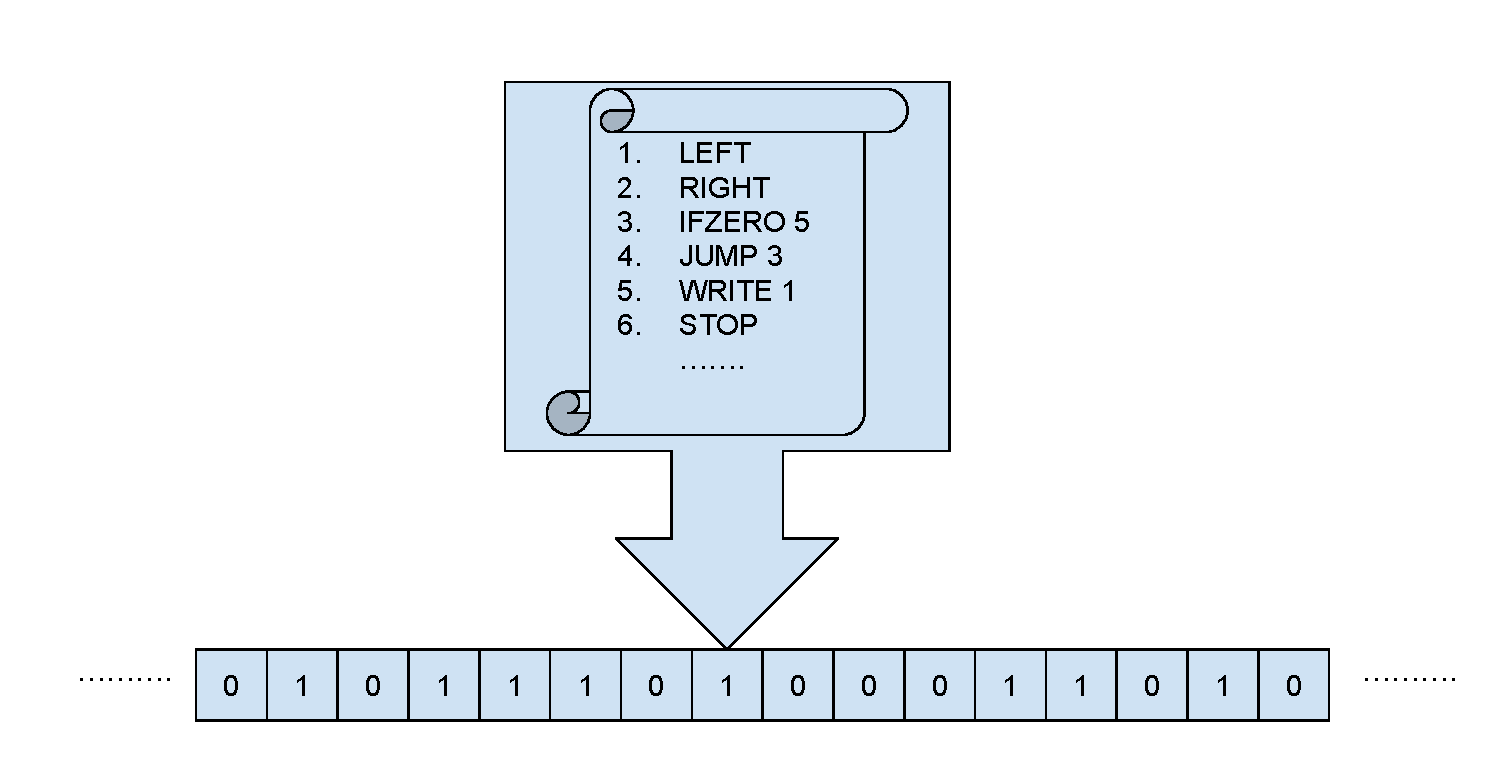
\includegraphics[width=0.9\textwidth]{images/turing.pdf}

  \pause
  \textbf{$M$ изчислява функцията $f_M$}, ако при лента с числото $n$ машината $M$ завършва и записва върху лентата числото $f_M(n)$.

  \pause
  Ако $M$ не завърши, казваме, че \textbf{$f_M(n)$ не е дефинирана}.
\end{frame}

\begin{frame}
  \frametitle{Езици за програмиране}
  \begin{itemize}[<+->]
  \item Машинни езици
    \begin{itemize}
    \item 20, 5, 2, 18, 7, 14, 12, 10, 3, 5, 23
    \end{itemize}
  \item Асемблерни езици
    \begin{itemize}
    \item \tt{ADD 5, 2}
    \item \tt{MOV 7, 14}
    \end{itemize}
  \item Макроезици
    \begin{itemize}
    \item \tt{add(\#5,2)}
    \item \tt{move(\#7,\#14)}
    \end{itemize}
  \item Процедурни езици
    \begin{itemize}
    \item \tt{a = a + 2; b = c;}
    \end{itemize}
  \item Структурни езици
    \begin{itemize}
    \item \tt{if (d > 3) d = c + 10;}
    \end{itemize}
  \item Декларативни езици
    \begin{itemize}
    \item \tt{f x = minimum [ y | y $\in$ [1..x], y${^2}$ $\geq$ x ]}
    \end{itemize}
  \end{itemize}
\end{frame}

\begin{frame}
  \frametitle{От код до програма}
  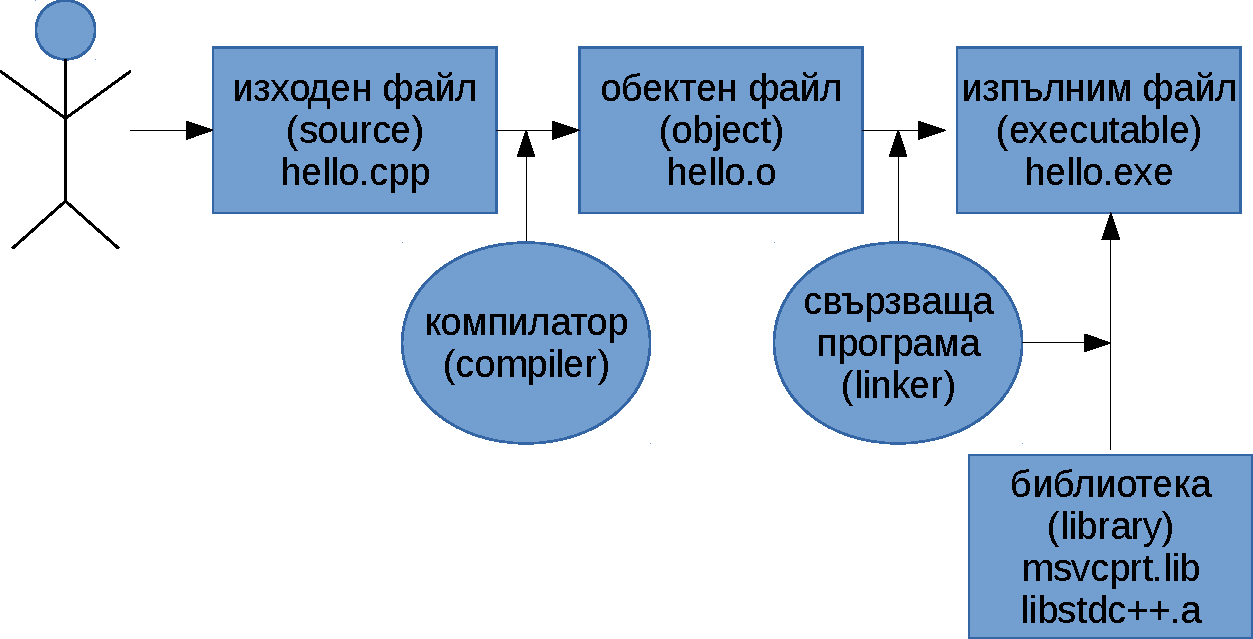
\includegraphics[width=0.9\textwidth]{images/compile.pdf}
\end{frame}

\begin{frame}[fragile]
  \frametitle{Първа програма на C++}
  \begin{lstlisting}
#include <iostream>
using namespace std;
int main() {
  int a = 5;
  cout << "a = " << a << endl;
  cout << "2a = " << 2 * a << endl;
  return 0;
}
  \end{lstlisting}
\end{frame}

\begin{frame}[fragile]
  \frametitle{Втора програма на C++}
\begin{lstlisting}
#include <iostream>
using namespace std;
int main() {
  int a, b;
  // първо въвеждаме стойности
  cout << "a = "; cin >> a;
  cout << "b = "; cin >> b;

  // събираме числата
  int c = a + b;

  // извеждаме резултата
  cout << "a + b = " << c << endl;
  return 0;
}
\end{lstlisting}
\end{frame}
\end{document}
